\documentclass[12pt,a4paper]{article}
\usepackage{fancyhdr}\usepackage{graphicx}\usepackage{placeins}\usepackage{adjustbox}
\begin{document}
\pagestyle{fancy}\fancyhf{}\chead{Short summary report}
\begin{table}[t]\centering\caption {rnaQUAST metrics for assembled transcripts. In each row the best values are indicated with \textbf{bold}. For the transcript metrics (rows 4, 5, 6, 9, 13, 27, 28, 29) we highlighted the best \textbf{relative} values i.e. divided by the total number of transcripts in the corresponding assembly.}\begin{adjustbox}{width=1\textwidth}\small\begin{tabular}{|l*{2}{|r}|}\hline\textbf{METRICS/TRANSCRIPTS}                            & \textbf{transcripts}   \\ \hline\hline
\multicolumn{2}{l}{\bf DATABASE METRICS}                                                  \\ \hline
Genes                                                   & 7126                   \\
Avg. number of exons per isoform                        & 1.06                   \\ \hline
\multicolumn{2}{l}{\bf BASIC TRANSCRIPTS METRICS}                                         \\ \hline
Transcripts                                             & 6511                   \\
Transcripts $>$ 500 bp                                  & \textbf{4448}          \\
Transcripts $>$ 1000 bp                                 & \textbf{3641}          \\ \hline
\multicolumn{2}{l}{\bf ALIGNMENT METRICS}                                                 \\ \hline
Aligned                                                 & \textbf{5933}          \\
Uniquely aligned                                        & 5800                   \\
Multiply aligned                                        & 59                     \\
Unaligned                                               & \textbf{578}           \\ \hline
\multicolumn{2}{l}{\bf ALIGNMENT METRICS FOR NON-MISASSEMBLED TRANSCRIPTS}                \\ \hline
Avg. aligned fraction                                   & \textbf{0.987}         \\
Avg. alignment length                                   & \textbf{1774.548}      \\
Avg. mismatches per transcript                          & \textbf{3.834}         \\ \hline
\multicolumn{2}{l}{\bf ALIGNMENT METRICS FOR MISASSEMBLED (CHIMERIC) TRANSCRIPTS}          \\ \hline
Misassemblies                                           & \textbf{48}            \\ \hline
\multicolumn{2}{l}{\bf ASSEMBLY COMPLETENESS (SENSITIVITY)}                               \\ \hline
Database coverage                                       & \textbf{0.74}          \\
Duplication ratio                                       & \textbf{1.028}         \\
50\%-assembled genes                                    & \textbf{3923}          \\
95\%-assembled genes                                    & \textbf{3634}          \\
50\%-covered genes                                      & \textbf{4012}          \\
95\%-covered genes                                      & \textbf{3756}          \\
50\%-assembled isoforms                                 & \textbf{3923}          \\
95\%-assembled isoforms                                 & \textbf{3634}          \\
50\%-covered isoforms                                   & \textbf{4012}          \\
95\%-covered isoforms                                   & \textbf{3756}          \\
Mean isoform coverage                                   & \textbf{0.951}         \\
Mean isoform assembly                                   & \textbf{0.933}         \\ \hline
\multicolumn{2}{l}{\bf GeneMarkS-T METRICS}                                               \\ \hline
Predicted genes                                         & \textbf{3825}          \\ \hline
\multicolumn{2}{l}{\bf ASSEMBLY SPECIFICITY}                                              \\ \hline
50\%-matched                                            & \textbf{604}           \\
95\%-matched                                            & \textbf{979}           \\
Unannotated                                             & \textbf{0.578}         \\ \hline
\end{tabular}\end{adjustbox}\end{table}
\FloatBarrier\clearpage\lfoot{generated by rnaQUAST}
\begin{figure}[t]\centering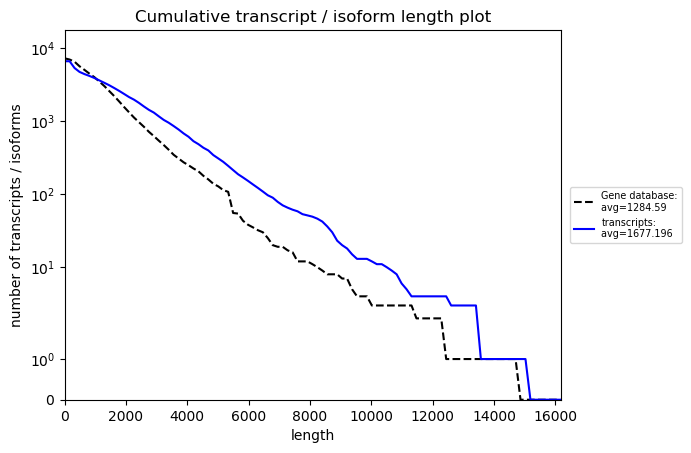
\includegraphics[width = \linewidth]{../../tools/rnaQUAST-2.0.1/rnaQUAST_results/results_2020_04_14_18_45_44/transcripts_output/transcript_length.png}\caption{Plot showing cumulative transcript length distribution. Each point represents the number of transcripts in the assembly with the corresponding length or longer; black dashed line corresponds to the database isoforms; the plot is given in logarithmic scale.}\end{figure}\FloatBarrier\clearpage
\begin{figure}[t]\centering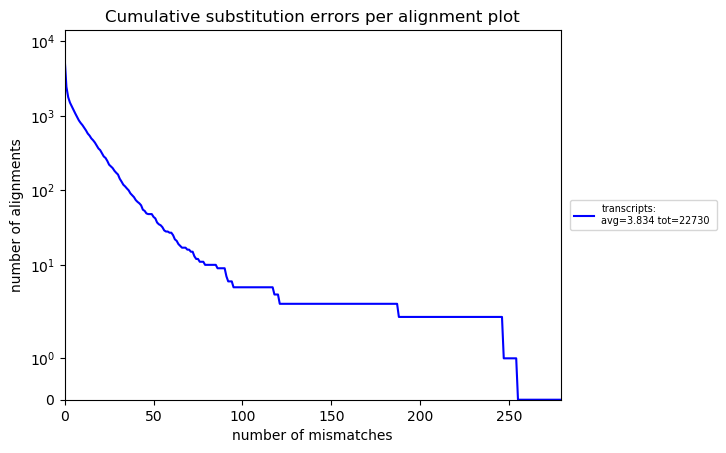
\includegraphics[width = \linewidth]{../../tools/rnaQUAST-2.0.1/rnaQUAST_results/results_2020_04_14_18_45_44/transcripts_output/mismatch_rate.png}\caption{Plot showing cumulative substitution errors per alignment distribution. Each point represents the number of alignments with the corresponding number of mismatches or greater; the plot is given in logarithmic scale.}\end{figure}\FloatBarrier\clearpage
\begin{figure}[t]\centering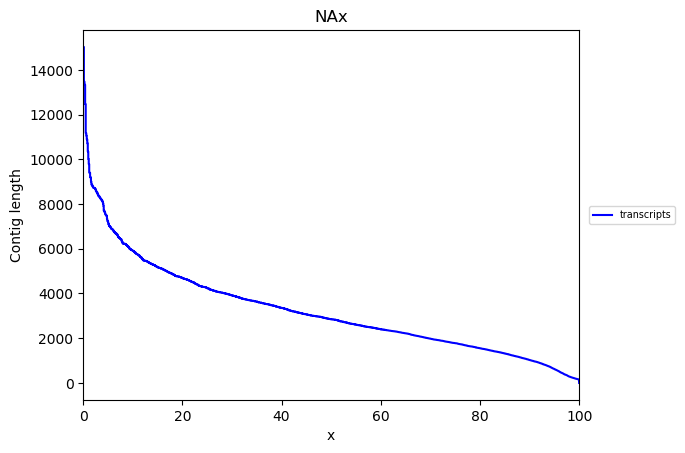
\includegraphics[width = \linewidth]{../../tools/rnaQUAST-2.0.1/rnaQUAST_results/results_2020_04_14_18_45_44/transcripts_output/NAx.png}\caption{Nx plot for transcripts. Nx is a maximal number $N$, such that the total length of all transcripts longer than $N$ bp is at least $x\%$ of the total length of all transcripts.}\end{figure}\FloatBarrier\clearpage
\begin{figure}[t]\centering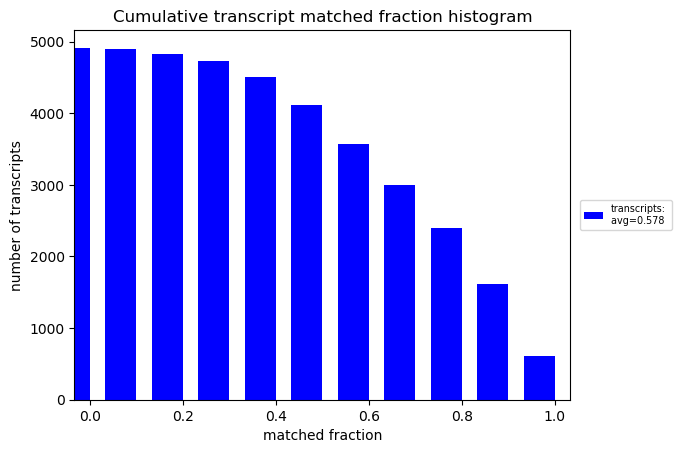
\includegraphics[width = \linewidth]{../../tools/rnaQUAST-2.0.1/rnaQUAST_results/results_2020_04_14_18_45_44/transcripts_output/x-matched.png}\caption{Plot showing cumulative transcript match histogram. Each bar represents the number of transcripts with matched fraction equal to or greater than the value on $x$ axis; transcript matched fraction is calculated as the number of its bases covering an isoform divided by the transcript length.}\end{figure}\FloatBarrier\clearpage
\begin{figure}[t]\centering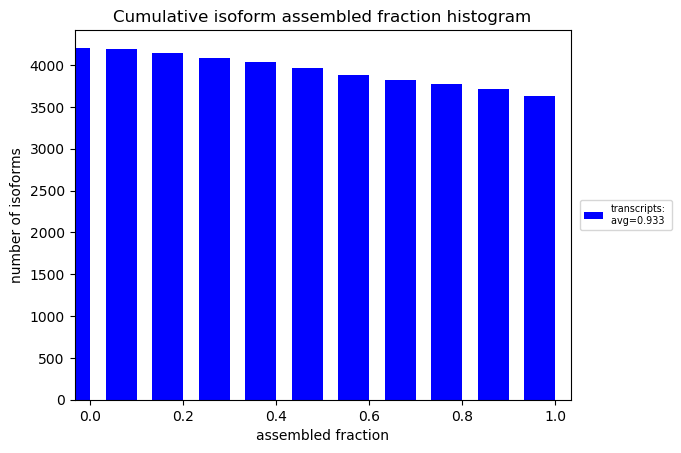
\includegraphics[width = \linewidth]{../../tools/rnaQUAST-2.0.1/rnaQUAST_results/results_2020_04_14_18_45_44/transcripts_output/x-assembled.png}\caption{Plot showing cumulative isoform assembly histogram. Each bar represents the number of isoforms with assembled fraction equal to or greater than the value on $x$ axis; isoform assembled fraction is calculated as the maximum number of captured by single assembled transcript bases divided by the total isoform length.}\end{figure}\FloatBarrier\clearpage
\begin{figure}[t]\centering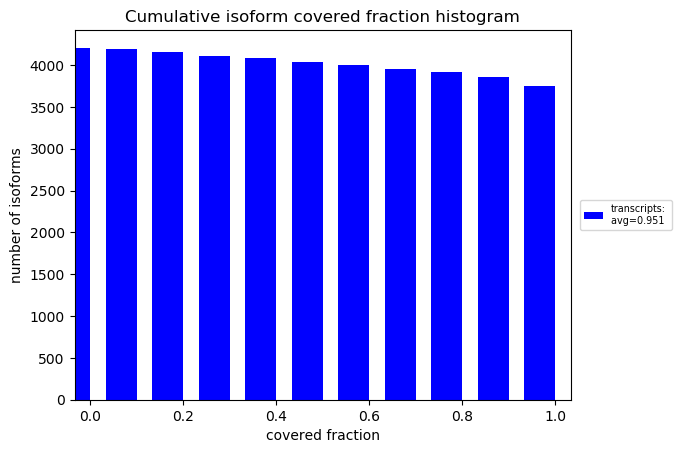
\includegraphics[width = \linewidth]{../../tools/rnaQUAST-2.0.1/rnaQUAST_results/results_2020_04_14_18_45_44/transcripts_output/x-covered.png}\caption{Plot showing cumulative isoform coverage histogram. Each bar represents the number of isoforms with covered fraction equal to or greater than the value on $x$ axis; isoform covered fraction is calculated as the number of covered bases (by all transcripts in the assembly) divided by the total isoform length.}\end{figure}\FloatBarrier\clearpage
\end{document}